by Polina Kozyr

\section{Porter's 5 Forces}

The idea behind Porter's model is that business profitability is influenced by several forces:

\begin{itemize}
\item Supplier power
\item Buying power
\item Competitive rivalry
\item Threat of new entry 
\item Threat of substitution
\end{itemize}
We developed a Porter's 5 Forces model for our product. The analysis is presented in table 5.1.

\begin{table}[ht]
    \centering
    \begin{tabular}{|c|c|c|}
        \hline
        \textbf{Force} & \textbf{Description} & \textbf{Threat level} \\
        \hline
        Buyer power &  \parbox{10cm}{\vspace{5pt}
            - Number of customers: large\\
            - Customers want smaller prices\\
            - Customers: elastic demand, not many alternatives, no switching costs\\
            - Businesses: elastic demand, not many alternatives, no switching costs\\
            - As the app operates on a subscription basis, users can easily switch to competitors if they are dissatisfied
            \vspace{5pt}} & Medium \\
    \hline
        Supplier power &  \parbox{10cm}{\vspace{5pt}
            -	Software suppliers: not that many suppliers, differentiation, but very stable, no switching costs
            \vspace{5pt}        
        } & Low \\
    \hline
        Competitive rivalry &  \parbox{10cm}{\vspace{5pt}
            -	Number of competitors: 3\\
            -	Multiple sensors systems with cameras: 0 competitors, this method can be more accurate but less easier in establishment\\
            -	Multiple sensors systems: 2 competitors\\
            -	Wearable sensors: accuracy depends on amount of sensors, but not all people want to wear something on them\\
            -	Solution with cameras: 1 competitors, similar to our solution\\
            -	no switching costs\\
            -	existing but not mature market\\
            -	brand image plays the role\\
            -	Product differentiation - medium
            \vspace{5pt}
            } & Medium \\
    \hline
        Threat of new entry &  \parbox{10cm}{\vspace{5pt}
            -	Modest profitability, slow growth\\
            -	advertisement requirement\\
            -	medical approval requirement\\
            -	brand identity is important\\
            -	economics of scale
            \vspace{5pt}
        } & Moderate \\
    \hline
        Threat of substitution &  \parbox{10cm}{\vspace{5pt}
            -	Multiple sensors systems: it's not easy to establish all equipment for customers, low threat\\
            -	Traditional Solutions: Traditional methods for improving posture, such as ergonomic chairs or physical therapy\\
            -	Other Health and Wellness Apps: Apps addressing general health and fitness may be substitutes, but the specific focus on posture control can mitigate this threat\vspace{5pt}
            \vspace{5pt}} & Low \\
    \hline
    \end{tabular}
    \caption{Porter's 5 Forces analysis}
\end{table}

\section{The Ansoff Matrix}

The Ansoff Matrix is presented in Figure 5.1.

\begin{figure}[H]
	\centering
	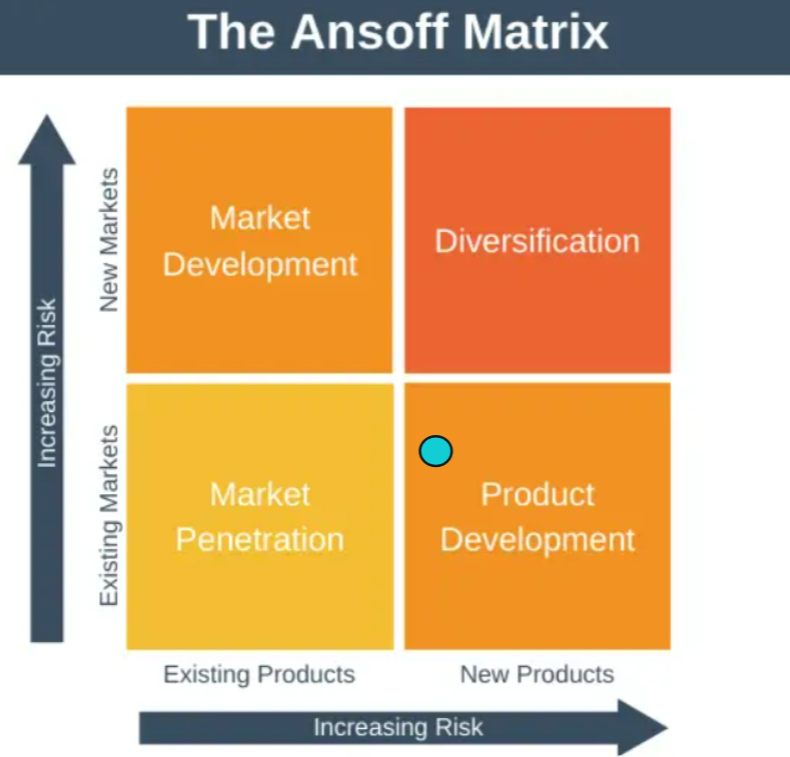
\includegraphics[width=0.7\textwidth]{figures/ansoff_matrix.png}
	\caption{The Ansoff Matrix}
	\label{fig:ansoff_matrix}
\end{figure}

The blue dot in the picture is our product. Therefore, we are going to work with the existing market - the German healthcare market. This market is existing but is not mature, so the risk is a little higher on this point. Our product is something between existing and new, since there are analogues and competitors, but there are just a very few of them and they are little known.

\section{Barriers to Entry and Exit}

Barriers to entry and exit are factors that can make it difficult for new firms to enter a particular industry or for existing firms to leave that industry. These barriers play a crucial role in shaping the competitive landscape of an industry and influencing the profitability of firms within it. In figure 5.2 you can see entry and exit risks for our posture controlling app that we can encounter. 

\begin{figure}[H]
	\centering
	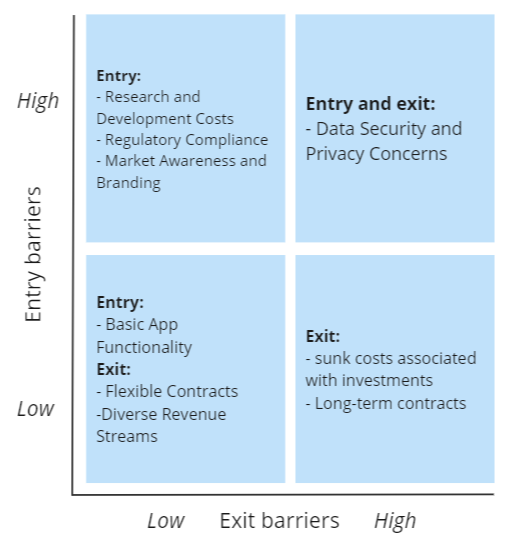
\includegraphics[width=0.6\textwidth]{figures/barriers_to_entry_and_exit.png}
	\caption{Barriers to Entry and Exit for posture controlling app development}
	\label{fig:barriers_to_entry_and_exit}
\end{figure}

\textbf{High barriers to entry}

\begin{itemize}
    \item Research and Development Costs: the significant investment needed for research, development, and testing creates a barrier. Larger companies or those with substantial financial backing may have an advantage over smaller entrants.
    \item Regulatory Compliance: compliance with health and privacy regulations adds complexity and cost to entry. 
    \item Market Awareness and Branding: building brand recognition and market awareness is a time-consuming and resource-intensive process. Established players with recognizable brands have a competitive advantage (e.g. Google).
    \item Technological Expertise: developing a sophisticated human posture-controlling app requires expertise in machine learning, and biomechanics. 
    \item Data Security and Privacy Concerns: establishing robust data security measures. 
\end{itemize}

\textbf{Low barriers to entry}
\begin{itemize}
\item Basic App Functionality: if the app's features are relatively basic and do not require highly specialized technology, it may be easier for new entrants to develop and offer similar solutions.
\end{itemize}

\textbf{High barriers to exit}
\begin{itemize}
\item Sunk Costs: investments in research, development, and infrastructure may face challenges exiting the market due to the significant sunk costs associated with these investments.
\item Long-term contracts with suppliers, partners, or employees can create obligations that make it difficult for a company to exit without incurring significant costs or legal consequences.
\item Data Security and Privacy Concerns: Exiting the market requires careful consideration of user data disposal, compliance with privacy regulations, and potential legal implications. Mishandling user data can result in legal consequences.
\end{itemize}

\textbf{Low barriers to exit}
\begin{itemize}
\item Flexible Contracts: having contracts with suppliers, partners, and employees that allow for flexibility and easy termination can lower exit barriers by minimizing contractual obligations.
\item Diverse Revenue Streams: companies with diversified revenue streams may find it easier to exit a particular market or product line without facing severe financial repercussions.
\end{itemize}


\section{Value chain}

In figure 5.3 you can see Value Chain analysis for our product.

\begin{figure}[H]
	\centering
	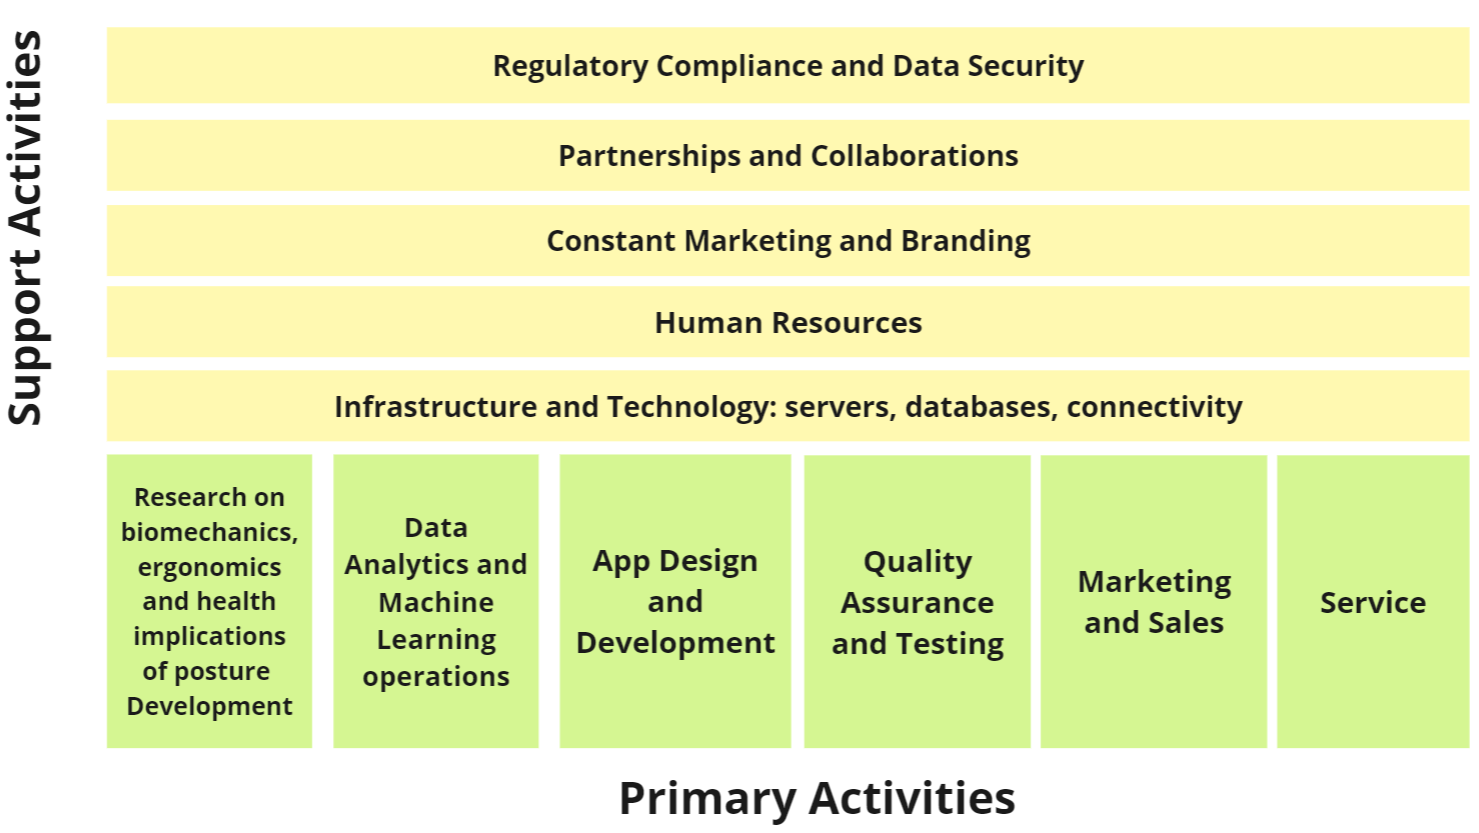
\includegraphics[width=1\textwidth]{figures/value_chain.png}
	\caption{Value chain analysis}
	\label{fig:value_chain}
\end{figure}

Primary activities are directly involved in the creation, delivery, and support of the product or service. They are essential for the production, marketing, and delivery of the final offering.\\

\textbf{Primary activities for our product:}
\begin{itemize}
    \item Research and Development

    Research on biomechanics, ergonomics, and health implications of posture. Development and enhancement of algorithms for real-time posture monitoring and feedback.
    \item Data Analytics and Machine Learning
    
    Analysis of posture data to provide personalized feedback and insights. Continuous improvement of machine learning algorithms for posture prediction and correction recommendations.
    \item App Design and Development
    
    Design of an intuitive and user-friendly interface for the app. Development of the app to ensure compatibility with various devices and operating systems.
    \item Quality Assurance and Testing
    
    Testing to ensure the accuracy and reliability of posture monitoring. We need to address any bugs or issues to enhance the overall user experience.
    \item Marketing and Sales
    
    Development of marketing strategies to promote the app, emphasizing its unique features and benefits. Implementation of sales channels, such as app stores or partnerships, to make the app accessible to users.
    \item Service
    
    This includes addressing customer inquiries, concerns, and issues related to the app. A responsive and helpful customer support team can enhance user experience and satisfaction.
\end{itemize}

Support activities provide the necessary infrastructure and resources to facilitate the primary activities. They don't directly contribute to the product but are crucial for the overall efficiency and effectiveness of the value chain.\\

\textbf{Support activities for our product:}
\begin{itemize}
    \item Infrastructure and Technology

    Management of the technological infrastructure, including servers, databases, and connectivity. We need to stay updated with emerging technologies that can enhance the app's performance.
    \item Human Resources

    Recruiting and training of more skilled personnel in areas such as software development, data analytics, and customer support.
    \item Partnerships and Collaborations

    Formation of partnerships with sensor manufacturers, health and wellness organizations, and other relevant entities. 
    \item Regulatory Compliance and Data Security:

    Implementation of robust data security measures to protect user information.
    \item Marketing and Branding:

    Engagement in marketing activities, including advertising, social media, and public relations efforts.
\end{itemize}